\documentclass[11pt,titlepage,fleqn]{article}

\usepackage{amsmath}
\usepackage{amssymb}
\usepackage{latexsym}
\usepackage[round]{natbib}
\usepackage{xspace}
\usepackage{graphicx}
\usepackage{epstopdf}
%\usepackage{epsfig}
\usepackage{float}
\usepackage{pifont}   % search for \ding

%\usepackage{fancyhdr}
%\pagestyle{fancy}

%=====================================================
%       SPACING COMMANDS (Latex Companion, p. 52)
%=====================================================

\usepackage{setspace}

%---------------------------
\newcommand{\matlab}{\textsc{Matlab}\xspace}
%---------------------------
\renewcommand{\baselinestretch}{1.0}

\textwidth 460pt
\textheight 700pt
\oddsidemargin 0pt
\evensidemargin 0pt

% see Latex Companion, p. 85
\voffset     -50pt
\topmargin     0pt
\headsep      20pt
\headheight    0pt
\footskip     30pt
\hoffset       0pt

\include{carlcommands}
%\input{dp_header}

\graphicspath{
  {/home/vipul/REPOSITORIES/IITR_seismo/classes/ES510/latex/figures/}
  }

\begin{document}

\noindent Course: Numerical Methods and Computer Programming\\
\noindent Code: ES 510\\
\noindent Instructor: Vipul Silwal (\verb+vsilwalfes@iitr.ac.in+) \\ 
\noindent Last Compiled: \today \\

{\huge Interpolation schemes}

\tableofcontents

%% ------------------------------------------------------------------------ %%
\section{Types of interpolation schemes}

\subsection{Piecewise constant interpolation}
or nearest neighbour interpolation
\begin{equation}
y = \begin{cases}
y_0 \,\,\, x < 0.5\\
y_1 \verb+ otherwise+
\end{cases}
\end{equation}

\begin{figure}[H]
\begin{tabular}{cc}
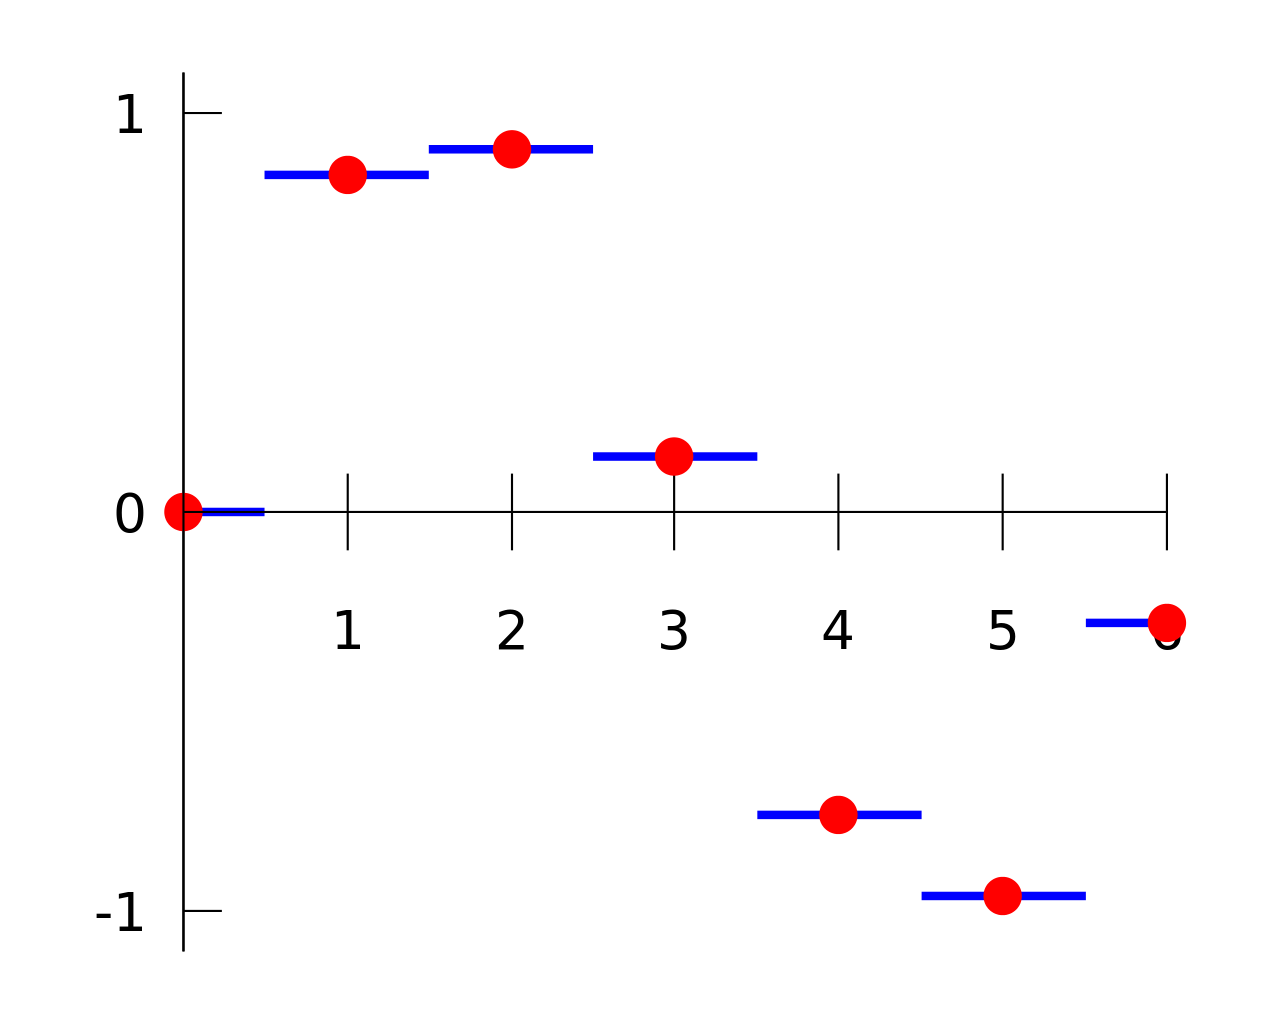
\includegraphics[scale=0.18]{piecewise_interp.png}&
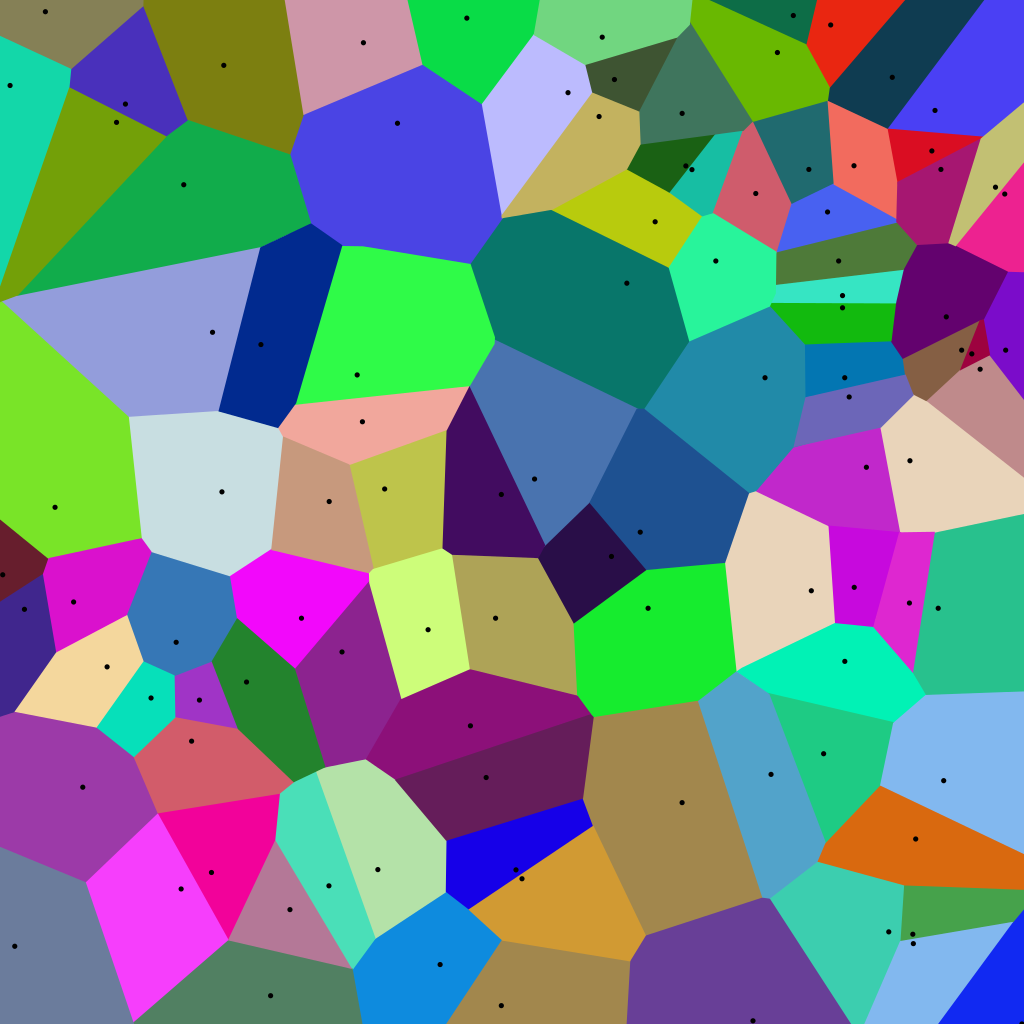
\includegraphics[scale=0.18]{piecewise_interp_voronoi.png}\\
\end{tabular}
\caption{(a) Piecewise interpolation on a set of discrete points. We can see that the resultant function is a discontinuous function. (b) Voronoi cells as an application of nearest neighbour interpolation. For a given set of points in space, a Voronoi diagram is a decomposition of space into cells, one for each given point, so that anywhere in space, the closest given point is inside the cell (source: wiki).}
\end{figure}

Examples of Voronoi discretization:
\begin{itemize}
\item Amazon storage house: For a particular delivery location find the nearest storage house. Steps: (1) Create Voronoi cell diagram using storage house as nodes; (2) Find the cell in which the location lies. (3) The node of that cell is your solution.
\item IITR Department-Bhawan allocation: Allocate nearest Bhawan to a particular department students. Steps: (1) Create Voronoi cell diagram using Department location as nodes; (2) Find the cell in which the Bhawans lie. (3) The node of that cell is your solution.
\end{itemize}

%------------------------------------------
\subsection{Linear interpolation}
\begin{equation}
y =  y_0 + (x - x_0) \frac{(y_1 - y_0)}{(x_1 - x_0)}
\end{equation}
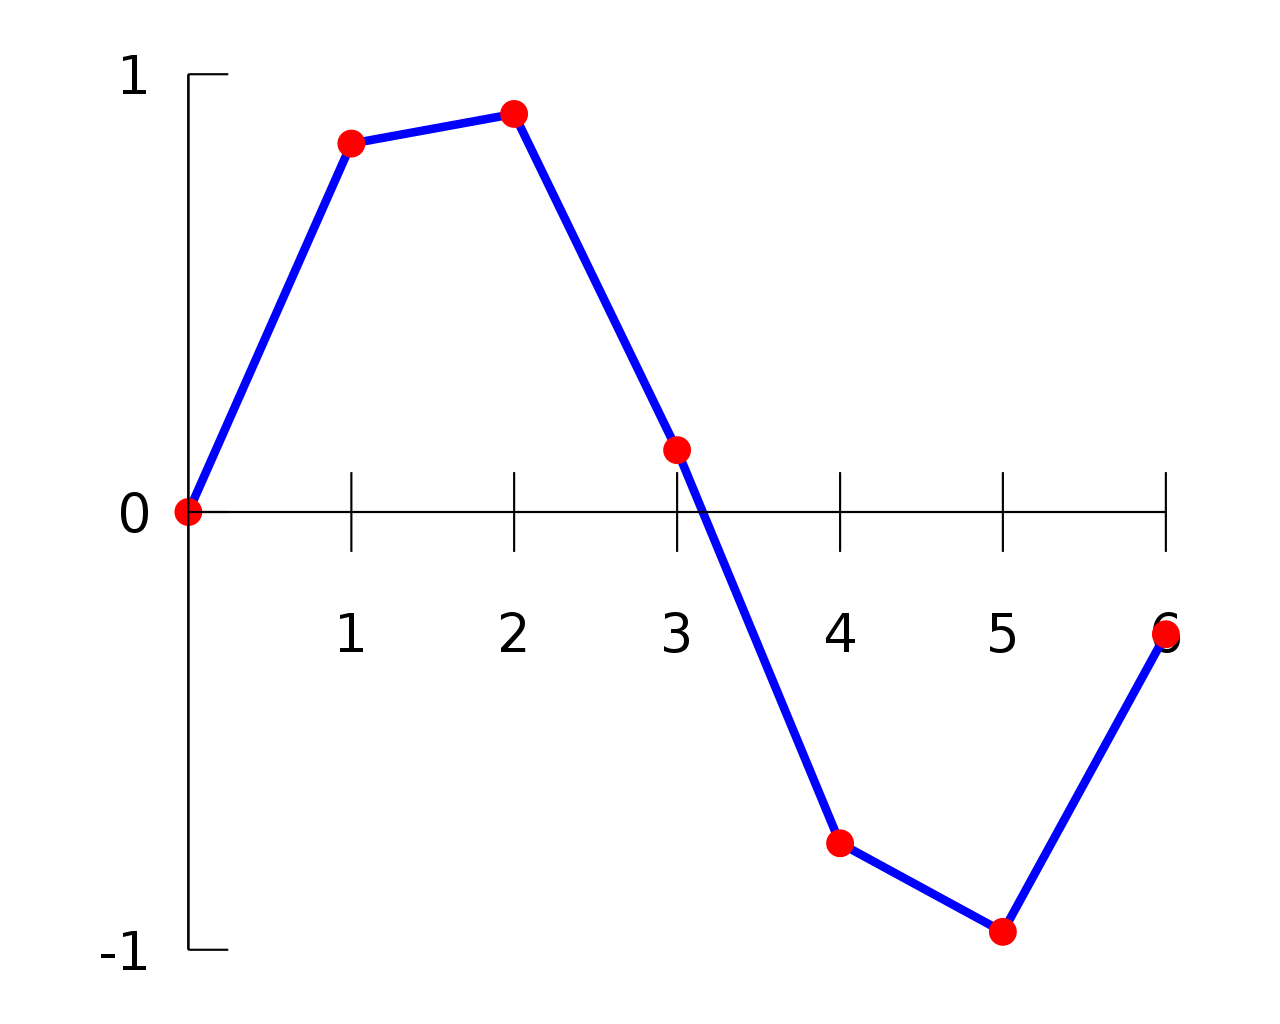
\includegraphics[scale=0.15]{linear_interp.png}

%------------------------------------------
\subsection{Polynomial interpolation}
\begin{equation}
y = a_0 + a_1x + a_2x^2 + \cdots + a_nx^n
\end{equation}

We need $n$-degree equation for interpolating N+1 points uniquely. For example, 3 independent points are needed to uniquely represent a quadratic equation. 

The resulting equations for $(x_i,y_i)$ is going to be:
\begin{eqnarray}
y_1 &=& a_0 + a_1x_1 + a_2x_1^2 + \cdots + a_nx_1^n\\
y_2 &=& a_0 + a_1x_2 + a_2x_2^2 + \cdots + a_nx_2^n\\
&\vdots& \\
y_n &=& a_0 + a_1x_n + a_2x_n^2 + \cdots + a_nx_n^n
\end{eqnarray}

We can represent this in matrix form as:
\begin{equation}
\begin{bmatrix}
1 & x_1 &  x_1^2  & \cdots & x_1^n\\
1 & x_2 & x_2^2 & \cdots & x_2^n\\
& & \vdots& &  \\
1 & x_n & x_n^2 & \cdots & x_n^n
\end{bmatrix}
\begin{bmatrix}
a_0 \\
a_1 \\
a_2 \\
\vdots\\
a_n\\
\end{bmatrix} = 
\begin{bmatrix}
y_0 \\
y_1 \\
y_2 \\
\vdots\\
y_n\\
\end{bmatrix} \label{eq:vandermonde}
\end{equation}

Matrix on the left is called a {\bf Vandermonde matix}. Such matrices generally have a large condition number and are hard to invert. Various optimization algorithms are adopted to get a stable solution.

Alternatively, one could directly obtain the interpolating polynomial using {\bf Lagrange polynomials}.

\begin{eqnarray}
p(x) &=& \frac{(x - x_1)(x - x_2)\cdots(x-x_n)}{(x_0 - x_1)(x_0 - x_2)\cdots(x_0-x_n)} y_0 + \frac{(x - x_0)(x - x_2)\cdots(x-x_n)}{(x_1 - x_0)(x_1 - x_2)\cdots(x_1-x_n)} y_1 +\\
&& \cdots +  \frac{(x - x_1)(x - x_2)\cdots(x-x_{n-1})}{(x_0 - x_1)(x_0 - x_2)\cdots(x_0-x_{n-1})} y_0\\
p(x) &=& \sum_{i=0}^n \left (\prod_{0\leq j\leq n, i\neq j} \frac{x-x_j}{x_i -x _j} \right ) y_i
\end{eqnarray}

%------------------------------------------
\section{Lagrange interpolation}
\verb+Notes from J.J. Westerink, University of Notre Dame+

Let there be $N+1$ points or the nodes such as $(x_0,y_0), (x_1,y_1), (x_2,y_2)... (x_N,y_N)$. We want to come up with some interpolating function $p(x)$ such that
\begin{eqnarray*}
p(x_0) &=& y_0 \\
p(x_1) &=& y_1 \\
&\vdots& \\
p(x_N) &=& y_N 
\end{eqnarray*}

Let us consider out interpolating function is of form:
\begin{equation}
p(x) = \sum_{i=0} y_i V_i(x)
\end{equation}

where $V_i$ are the lagrange polynomials with $y_i$ being the coefficients.

We would like $V_i$ to have the following property:
\begin{equation}
V_i(x_j) =  \begin{cases}
0 \,\,\, i\neq j\\
1 \,\,\, i=j
\end{cases} \label{eq:lagrange_cases}
\end{equation}

which would force the interpolating function $p(x)$ to be equal to $y_i$ at every node point.

For example for 5 interpolating nodes:
\begin{equation}
p(x_3) = y_0V_0(x_3) + y_1V_1(x_3) + y_2V_2(x_3) + y_3V_3(x_3) + y_4V_4(x_3)
\end{equation}

Using the constrain from equation \refeq{lagrange_cases} this would condense down to $p(x_3) = y_3$.
\linebreak

{\bf Properties of $V_i(x)$}
\begin{enumerate}
\item Degree $N$
\item Roots at $x_0, x_1,....x_{i-1}, x_{i+1},...x_N$ (all nodes except $x_i$)
\item $V_i(x_i) = 1$
\end{enumerate}

The following function satisfies the first two properties:
\begin{equation}
W_i(x) = (x-x_0) (x-x_1)(x-x_2) \cdots (x-x_{i-1})(x-x_{i+1})\cdots(x-x_N)
\end{equation}
The third property could be satisfied by normalizing the function:
\begin{equation}
V_i(x) = \frac{(x-x_0) (x-x_1)(x-x_2) \cdots (x-x_{i-1})(x-x_{i+1})\cdots(x-x_N)}{(x_i-x_0) (x_i-x_1)(x_i-x_2) \cdots (x_i-x_{i-1})(x_i-x_{i+1})\cdots(x_i-x_N)}
\end{equation}

This could be written in a condensed form as:
\begin{equation}
V_i(x) = \prod_{0\leq j\leq n} \left (\frac{x-x_j}{x_i -x _j} \right )
\end{equation}

So our final interpolation function is:
\begin{equation}
p(x) = \sum_{i=0} y_i V_i(x) = \sum_{i=0}^n y_i \left (\prod_{0\leq j\leq n, i\neq j} \frac{x-x_j}{x_i -x _j} \right )
\end{equation}

%-------------------------------------------
\subsection{Connection between Vandermonde matrix and Lagrange polynomials}

Starting with \refeq{eq:vandermonde} and then taking in the inverse of the Vandermonde matrix (the \bG of in equation $\bd = \bG \bem$).

\begin{equation}
\begin{bmatrix}
1 & x_1 &  x_1^2  & \cdots & x_1^n\\
1 & x_2 & x_2^2 & \cdots & x_2^n\\
& & \vdots& &  \\
1 & x_n & x_n^2 & \cdots & x_n^n
\end{bmatrix}
\begin{bmatrix}
a_0 \\
a_1 \\
a_2 \\
\vdots\\
a_n\\
\end{bmatrix} = 
\begin{bmatrix}
y_0 \\
y_1 \\
y_2 \\
\vdots\\
y_n\\
\end{bmatrix}
\end{equation}

\begin{equation}
\begin{bmatrix}
a_0 \\
a_1 \\
a_2 \\
\vdots\\
a_n\\
\end{bmatrix} = 
\begin{bmatrix}
1 & x_1 &  x_1^2  & \cdots & x_1^n\\
1 & x_2 & x_2^2 & \cdots & x_2^n\\
& & \vdots& &  \\
1 & x_n & x_n^2 & \cdots & x_n^n
\end{bmatrix}^{-1}
\begin{bmatrix}
y_0 \\
y_1 \\
y_2 \\
\vdots\\
y_n\\
\end{bmatrix}
\end{equation}

\begin{equation}
\begin{bmatrix}
a_0 \\
a_1 \\
a_2 \\
\vdots\\
a_n\\
\end{bmatrix} = 
\begin{bmatrix}
V_0(x_0) & V_1(x_0) &  V_2(x_0)  & \cdots & V_N(x_0)\\
V_0(x_1) & V_1(x_1) &  V_2(x_1)  & \cdots & V_N(x_1)\\
& & \vdots& &  \\
V_0(x_N) & V_1(x_N) &  V_2 (x_N) & \cdots & V_N(x_N)\\
\end{bmatrix}
\begin{bmatrix}
y_0 \\
y_1 \\
y_2 \\
\vdots\\
y_n\\
\end{bmatrix}
\end{equation}

%===========================================
\section{Exercises}
\begin{enumerate}
\item Consider there are 10 randomly distributed Amazon storage location in a $100 \times 100$ km area. Create a Voronoi cell diagram using storage locations as nodes. Randomly select 5 location points and their nearest distribution store. [Hint: Use matlab's \verb+randn, voronoi+ functions].
\end{enumerate}

\end{document}
